\documentclass[12pt]{article}
\usepackage{amsmath}
\usepackage{amssymb}
\usepackage{geometry}
\usepackage{enumerate}
\usepackage{natbib}
\usepackage{float}%稳定图片位置
\usepackage{graphicx}%画图
\usepackage[english]{babel}
\usepackage{a4wide}
\usepackage{indentfirst}%缩进
\usepackage{enumerate}%加序号
\usepackage{multirow}%合并行
\title{\large UM-SJTU JOINT INSTITUTE\\PHYSICS LABORATORY\\(VP141)\\\ \\\ \\\ \\\ \\\ \\\ \\\ \\\ \\\ \\\ \\\
LABTORATORY REPORT\\\ \\\ EXERCISE 1\\\  Measurements of the Moment of Inertia \\\ \\\ \\\ \\\ \\\ }
\author{Name: Pan Chongdan\\ID: 516370910121\\Group: 16}
\date{Date: \today}

\begin{document}
\maketitle
\newpage
\section{Introduction and Theoretical Background}
\subsection{Objectives}
The main objective of this exercise is to get familiar with the constant-torque method for measuring the moment of inertia of a rigid body. Student will study the dependence of the moment of inertia on mass distribution and on the choice of the rotation axis. The parallel axis (Steiner's) will be verified in this exercise as well. Student's measurement technique skills will also be developed by learning how to measure time using a photo-gate electronic timer.
\subsection{Basic Concepts of moment of inertia}
A rigid body's moment of inertia about an axis is a quantitative characteristics that denes the body's resistance (inertia) to a change of angular velocity in rotation about that axis. The moment of inertia of a rigid body rotating about a fixed axis is determined not only by the mass of the body, but also by its distribution. The moment of inertia of a rigid body about a certain rotation axis can be calculated analytically as long as the body has regular shape or uniformly distributed mass. Otherwise, the calculation may be difficult. Experimental methods turn out to be more useful in such cases.
\par For rigid body which has an irregular shape or non-uniformly distributed mass, its moment of inertia can be expressed as following equation
\begin{equation}
I=m_1r_1^2+m_1r_2^2+\cdots+\sum_{i} m_ir_i^2
\end{equation}
{\centering \footnotesize  I:Moment of Inertia of a body for a given rotation axis\\
$m_i$:Masses of the particles making up the body \\$r_i$:Perpendicular distances of the particles from rotation axis\\
}
\subsection{Second Law of Dynamics for Rotational Motion}
According to the second law of dynamics for rotational motion about a fixed axis 
\begin{equation}
\tau_z =I\beta_z    
\end{equation} 
\noindent relates the component of the torque $\tau_z$ about the axis of rotation with the moment of inertia about this axis, and the angular acceleration component $\beta_c$. Therefore, the moment of inertia I can be found once the torque and the resulting angular acceleration are measured.
\par The moment of inertia is an additive quantity, i.e. if the moment of inertia of a rigid
body (A) about an axis is $I_A$ and the moment of inertia of another rigid body (B) about the same axis is $I_B$, then the moment of inertia of the combined rigid body AB composed of A and B, about the same axis of rotation, is 
\begin{equation}
I_{AB}=I_A+I_B
\end{equation}	
\subsection{Parallel Axis Theorem}
If the moment of inertia of a rigid body with mass m about an axis through the body's
center of mass is $I_0$, then for any axis parallel to that axis, the moment of inertia is
\begin{equation}
I=I_0+md^2 
\end{equation} 
where d is the distance between the axes. This result is known as the parallel axis theorem
or Steiner's theorem.
\section{Measurement Setup and Measurement Method}
\subsection{Measurement of the Moment of Inertia}
The measurement setup is shown in Figure 1. It consists of a turntable with an integrated photo-gate system used for time measurements.
\par In order to understand the idea of the measurement method, suppose that the empty
turntable is initially rotating and its moment of inertia with respect to the rotation axis
is $I_1$. Since the bearings of the turntable are not frictionless, there will be a non-zero
frictional torque $M_\mu$ causing the turntable to decelerate with angular acceleration $\beta_1$,
so that the second law of dynamics for rotational motion of the empty turntable reads
(furthermore we will skip the subscript $\mathit{z}$)
\begin{equation}
M_\mu =-I_1\beta_1    
\end{equation} 
\begin{figure}[H]
\centering
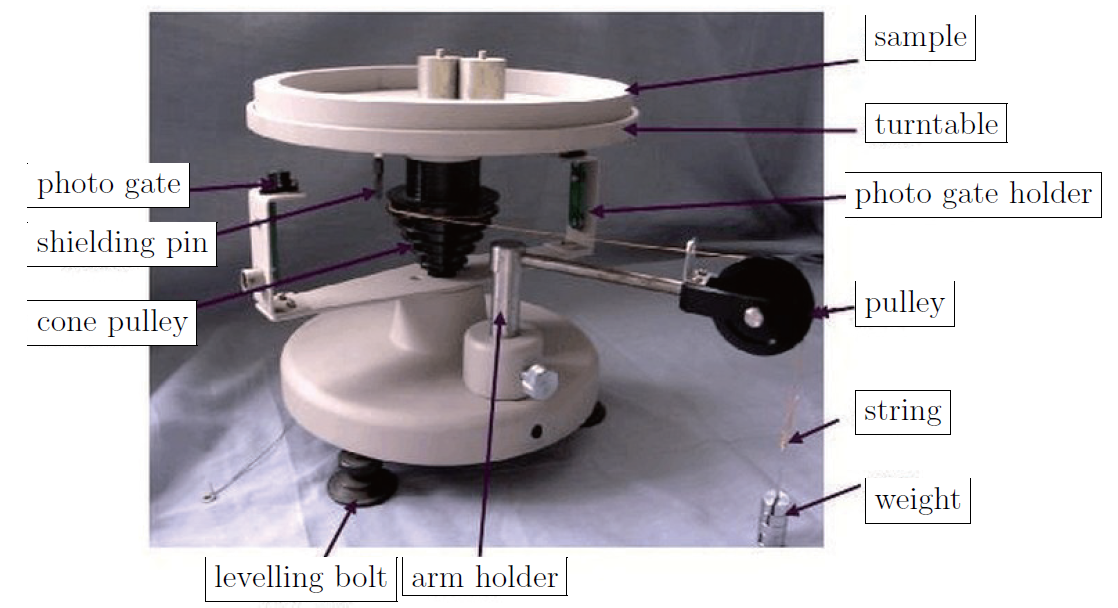
\includegraphics[width=1\linewidth]{setup.jpg}
\caption{\label{fig:measurement setup}Measurement Setup.}
\end{figure}
\par Below the turntable, there is a conical pulley of radius $R$, with a light and inextensible
string wound on it. The axis of the cone coincides with the axis of rotation. Attached to
the other end of the string passing through a disk pulley, there is a weight with mass m,
free to move downwards after it is released. If the mass moves downwards with constant
acceleration a, the tension in the string T is constant and $T = m(g-\mathit{a})$. This constant
tension force, on the other end of the string, provides constant torque on the cone pulley
that in turn makes the turntable rotate the with constant angular acceleration. If the
turntable rotates with angular acceleration $\beta_2$, then $a = R\beta_2$ (we assume that the string does not slip on the pulleys). The torque the string exerts on the pulley (and hence the turntable) is then $TR = m(g-R\beta_2)R$. Consequently, taking into account the frictional torque, the net torque on the turntable is $TR-M_\mu$, and the equation of motion for the turntable reads
\begin{equation}
m(g-R\beta_2)R-M_\mu=I_1\beta_2
\end{equation}
Eliminating $M_\mu$ from Eqs. (3) and (4), we find
\begin{equation}
I_1=\frac{mR(g-R\beta_2)}{\beta_2-\beta_1}
\end{equation}
\par Similarly, if a rigid body with an unknown moment of inertia is placed on the turntable,
we may find
\begin{equation}
I_2=\frac{mR(g-R\beta_4)}{\beta_4-\beta_3}
\end{equation}
where $\beta_3$ is the magnitude of angular deceleration of the turntable with the body, and $\beta_3$ is its angular acceleration, when the mass m is released and moves downwards.
\par Using the fact that the moment of inertia is an additive quantity, the moment of inertia
of the rigid object placed on the turntable, with respect to the axis of rotation, may be
found as the difference
\begin{equation}
I_3=I_2-I_1
\end{equation}
\subsection{Measurement of Angular Acceleration}
At the edge of the turntable two shielding pins are fixed. As the turntable rotates,
the pins generate a series of signals in the photo-gate with the phase interval of $\pi$. An
integrated counter-type electronic timer is used to measure the consecutive number $k$ and
the time $t$ of the photo-gate signal.
\par If (k,t) is a set of the measurement data, the corresponding angular position is
\begin{equation}
\theta=k\pi=\omega_0t+\frac{1}{2}\beta t^2
\end{equation}
where $\omega_0$ is the initial angular speed. Now, by performing a quadratic fit to the measurement data, we can find the angular acceleration.
\section{Apparatus}
As shown in the measurement setup part,we have many apparatus in our exercise. I classify them into two parts. 
\subsection{Tools} The first part is tools, including the electronic timer, vernier calliper, and electronic balance. However, the tools have their limit of precision, which may cause systematic errors in my results. 
\begin{figure}[H]
\centering
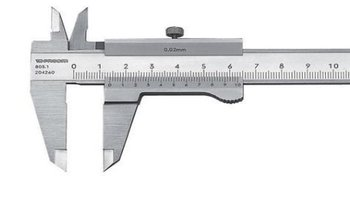
\includegraphics[width=0.7\linewidth]{Calliper.jpg}
\caption{\label{fig:Calliper}Calliper.}
\end{figure} 
\begin{table}[H]
\centering
\begin{tabular}{cllll}
\cline{1-4}
\multicolumn{1}{|r|}{\textbf{}} & \multicolumn{1}{l|}{Calliper} & \multicolumn{1}{l|}{Electronic balance} & \multicolumn{1}{l|}{Timer} &  \\ \cline{1-4}
\multicolumn{1}{|c|}{Resolution} & \multicolumn{1}{c|}{0.002cm} & \multicolumn{1}{c|}{0.1g} & \multicolumn{1}{c|}{0.0001s} &  \\ \cline{1-4}
\multicolumn{1}{|c|}{Relative uncertainty} & \multicolumn{2}{c|}{/} & \multicolumn{1}{c|}{0.004\%} &  \\ \cline{1-4}
\multicolumn{1}{l}{} &  &  &  & 
\end{tabular}
\caption{Precision of the measurement instruments}
\end{table}
\subsection{Materials}
The second part is materials that we use and measure to help us indirectly examine the moment of inertia. The materials include one Disk, two hoops of different radiant, two similar cylinders, one cone pulley, and one weight.
\par In this experiment, I need to measure the moment of inertia of the empty turntable, the hoop, the disk and the cylinder, as well as verify the parallel-axis theorem by placing two cylinders off the axis while keeping their center of mass on the axis in order to keep the rotation steady. The distances between the holes and the center of the turntable are 45, 60, 75, 90, 105 mm, respectively.
\section{Measurement Procedure}
\begin{enumerate}
\item  Measure the mass of the weight, the hoop, the disk, and the cylinder, as well as
the radius of the cone pulley and the cylinder (follow the instructor's requirements).
Calculate the moment of inertia of the hoop and the disk analytically.
Use a reliable source to find the local value of the acceleration due to gravity in
Shanghai.
\item Turn the electronic timer on and switch it to mode 1-2 (single gate, multiple pulses).
\item Place the instrument close to the edge of the desk and stretch the disk pulley arm
outside, so that the weight can move downwards unobstructed.
\item Level the turntable with the bubble level.
\item Make the turntable rotating and press the start button on the timer. After at least
8 signals are recorded, stop the turntable and record the data in your data sheet.
\item Attach the weight to one end of the string. Place the string on the disk pulley,
thread through the hole in the arm, and wind the string around the 3rd ring of the
cone pulley. Adjust the arm holder so that the string goes through the center of the
hole.
\item Release the weight and start the timer. Stop the turntable when the weight hits the
floor. Write down the recorded data.
\item The angular acceleration can be found by plotting $\theta= k\pi$ against $t$ and performing a quadratic fit using data processing software. (The magnitude of the angular
acceleration is equal to the coefficient next to $t^2$ multiplied by two. The uncertainty
of the angular acceleration can be read directly from the fitting result.)
The moment of inertia of the empty turntable is found by using the formulae in
Section 3 and the data from step 5 and 7. Repeat steps $5\thicksim7$ with a rigid object
placed on the turntable. Eq. (7) is used to find the moment of inertia of the rigid
object.
\par In the experiment, each student should measure the moment of inertia of the empty
turntable, the hoop, the disk and the cylinder, as well as verify the parallel-axis theorem by placing two cylinders of the axis while keeping their center of mass on the axis in
order to keep the rotation steady.
\par The distances between the holes and the center of the turntable are ca. 45, 60, 75, 90,
105 mm, respectively. The timer's resolution is 0:0001 s, and the error is 0:004%.
\end{enumerate}
\section{Calculation and Results}
\subsection{Relative Parameters of Materials}
	In the exercise, I use a calliper to measure the diameter of the disk, the inner diameter and external diameter of two hoops, the two cylinder's diameter, the cone pulley's diameter and distance between the holes that I choose.
	\begin{table}[H]
\centering
\begin{tabular}{|r|c|c|c|l|}
\hline
\multicolumn{1}{|l|}{}                       & 1      & 2      & 3      & \multicolumn{1}{c|}{4} \\ \hline
Disk $\varnothing$ {[}cm{]} $\pm$ 0.002{[}cm{]}               & 23.988                 & 24.000                 & 24.002                 & 24.010 \\ \hline
Hoop $\varnothing_1${[}cm{]} $\pm$ 0.002{[}cm{]}             & 21.380                 & 21.388                 & 21.224                 & 21.404 \\ \hline
Hoop $\varnothing_2${[}cm{]} $\pm$ 0.002{[}cm{]}              & 23.596                 & 23.620                 & 23.640                 & 23.542 \\ \hline
Cylinder A $\varnothing$ {[}cm{]} $\pm$ 0.002{[}cm{]}         & 3.000                  & 2.996                  & 2.992                  & 2.984  \\ \hline
Cylinder B $\varnothing$ {[}cm{]} $\pm$ 0.002{[}cm{]}         & 2.996                  & 2.986                  & 2.988                  & 2.986  \\ \hline
Cone pulley $\varnothing$ {[}cm{]} $\pm$ 0.002{[}cm{]}        & 5.014                  & 5.020                  & 5.010                  & 5.014  \\ \hline
Hole \textcircled{1} d {[}cm{]} $\pm$ 0.002{[}cm{]}   & 4.002                  & 5.014                  & \multicolumn{2}{c|}{/}          \\ \hline
Hole \textcircled{2} d {[}cm{]} $\pm$ 0.002{[}cm{]} & 3.992                  & 5.024                  & \multicolumn{2}{c|}{/}          \\ \hline
Hole \textcircled{3} d {[}cm{]} $\pm$ 0.002{[}cm{]} & 5.482                  & 6.504                  & \multicolumn{2}{c|}{/}          \\ \hline
Hole \textcircled{4} d {[}cm{]} $\pm$ 0.002{[}cm{]} & 5.488                  & 6.482                  & \multicolumn{2}{c|}{/}          \\ \hline
\end{tabular}
\caption{Calliper measurements.}
\end{table}
The hole numbers is consistent with my choice in table 4. The distance of the hole to the rotation center is measured as: the inner distance and the outer distance. Other parameters are measured 4 times.
\par In addition, I also use the electronic balance to measure the mass of disk, hoop, two cylinders and the weight
\begin{table}[H]
\centering
\begin{tabular}{|r||r|r|l|}
\hline
Disk {[}g{]} $\pm$ 0.1{[}g{]}       & 490.2 & Hoop {[}g{]} $\pm$ 0.1{[}g{]}     & 429.4 \\ \hline
Cylinder A {[}g{]} $\pm$ 0.1{[}g{]} & 166.0 & Cylinder B {[}g{]} $\pm$ 0.1{[}g{]} & 165.9 \\ \hline
Weight {[}g{]} $\pm$ 0.1{[}g{]}     & 54.5  &                                   &       \\ \hline
\end{tabular}
\caption{Mass measurements}
\end{table}  
\subsection{Theoretical Moment of inertia of Disk, Hoops and Cylinders }
Since I've measure the relative parameter of the materials, they will be used to calculate the theoretical value of moment of inertia
\subsubsection{Theoretical Moment of Inertia of the Disk}
$$R_{disk}=\frac{1}{2}\bar{\varnothing}_{disk}=12.000\pm0.008[cm]$$
$$I_{disk}=\frac{1}{2}M_{disk}R^2_{disk}=3.529\times10^{-3}\pm4.47\times10^{-6}[kg\cdot{m^2}]$$
\subsubsection{Theoretical Moment of Inertia of Hoops}
$$R_{hoop1}=\frac{1}{2}\bar{\varnothing_1}=10.675\pm0.066[cm]$$
$$R_{hoop2}=\frac{1}{2}\bar{\varnothing_2}=11.800\pm0.034[cm]$$
The moment of inertia of the hoop is estimated by:
$$I_{hoop}=\frac{1}{2}M_{hoop}(R^2_{hoop1}+R^2_{hoop2})=5.435\times10^{-3}\pm3.66\times10^{-5}[kg\cdot{m^2}]$$
\subsubsection{Theoretical Moment of Inertia after cylinders are added}
The cylinders' radius are:
$$R_{A}=\frac{1}{2}\bar{\varnothing}_{A}=1.497\pm0.006[cm]$$
$$R_{B}=\frac{1}{2}\bar{\varnothing}_{B}=1.495\pm0.004[cm]$$
If they're rotating around the their center, their moment of inertia are:
$$I_{A}=\frac{1}{2}m_{A}R^2_{A}=1.860\times10^{-5}\pm9.797\times10^{-8}[kg\cdot{m^2}]$$
$$I_{B}=\frac{1}{2}m_{B}R^2_{B}=1.853\times10^{-5}\pm6.907\times10^{-8}[kg\cdot{m^2}]$$
The distance from the four holes to the center are:\\
$$d_1=4.508\pm0.0014[cm]$$
$$d_2=4.508\pm0.0014[cm]$$
$$d_3=5.993\pm0.0014[cm]$$
$$d_4=5.985\pm0.0014[cm]$$
Then according to Parallel Axis Theorem\\
If cylinder A and cylinder B are placed in hole \textcircled{1} and hole \textcircled{2} respectively,
$$I_{A1B2}=I_A+m_Ad_1^2+I_B+m_Bd_2^2=7.116\times10^{-4}\pm1.6\times10^{-5}[kg\cdot{m^2}]$$
If cylinder A and cylinder B are placed in hole \textcircled{3} and hole \textcircled{4} respectively,
$$I_{A3B4}=I_A+m_Ad_3^2+I_B+m_Bd_4^2=1.228\times10^{-3}\pm5.06\times10^{-7}[kg\cdot{m^2}]$$
\subsection{Measurement of the Moment of Inertia}
I use constant-torque method to find the moment of inertia in this exercise. To calculate the moment of inertia, I've already measured following physical quantities:
\begin{center}
The acceleration due to gravity: $g=9.7494\pm0.001[m/s^2]$\\
The mass of the weight: $m=54.5\pm0.1[g]$\\
The radius of the cone pulley: $R_{cone}=\frac{1}{2}\bar{\varnothing_cone}=2.508\pm0.035[cm]$
\end{center}
\begin{table}[H]
\centering
\begin{tabular}{|c|c|c|c|c|l||c|c|c|c|c|}
\hline
\multirow{5}{*}{\begin{tabular}[c]{@{}c@{}}Empty\\ turntable\end{tabular}} & \multicolumn{5}{c||}{Deceleration}                                                                          & \multicolumn{5}{c|}{Acceleration}                                                                                          \\ \cline{2-11} 
                                                                           & \multicolumn{1}{l|}{k} & \multicolumn{1}{l|}{1} & \multicolumn{1}{l|}{2} & \multicolumn{1}{l|}{3} & 4      & \multicolumn{1}{l|}{k} & \multicolumn{1}{l|}{1} & \multicolumn{1}{l|}{2} & \multicolumn{1}{l|}{3} & \multicolumn{1}{l|}{4} \\ \cline{2-11} 
                                                                           & t {[}s{]}              & 1.1452                 & 2.3156                 & 3.5037                 & 4.7182 & t {[}s{]}              & 0.8993                 & 1.5529                 & 2.0941                 & 2.5797                 \\ \cline{2-11} 
                                                                           & \multicolumn{1}{l|}{k} & \multicolumn{1}{l|}{5} & \multicolumn{1}{l|}{6} & \multicolumn{1}{l|}{7} & 8      & \multicolumn{1}{l|}{k} & \multicolumn{1}{l|}{5} & \multicolumn{1}{l|}{6} & \multicolumn{1}{l|}{7} & \multicolumn{1}{l|}{8} \\ \cline{2-11} 
                                                                           & t {[}s{]}              & 5.9521                 & 7.2158                 & 8.5009                 & 9.8189 & t {[}s{]}              & 3.0134                 & 3.4372                 & 3.8926                 & 4.4138                 \\ \hline
\multirow{5}{*}{\begin{tabular}[c]{@{}c@{}}With disk\end{tabular}} & \multicolumn{5}{c|}{Deceleration}                                                                          & \multicolumn{5}{c|}{Acceleration}                                                                                          \\ \cline{2-11} 
                                                                           & \multicolumn{1}{l|}{k} & \multicolumn{1}{l|}{1} & \multicolumn{1}{l|}{2} & \multicolumn{1}{l|}{3} & 4      & \multicolumn{1}{l|}{k} & \multicolumn{1}{l|}{1} & \multicolumn{1}{l|}{2} & \multicolumn{1}{l|}{3} & \multicolumn{1}{l|}{4} \\ \cline{2-11} 
                                                                           & t {[}s{]}              & 1.0060             & 2.0264                 & 3.0550                 & 4.0988 & t {[}s{]}              & 2.0963                 & 3.3393                 & 4.2880               & 5.0304                \\ \cline{2-11} 
                                                                           & \multicolumn{1}{l|}{k} & \multicolumn{1}{l|}{5} & \multicolumn{1}{l|}{6} & \multicolumn{1}{l|}{7} & 8      & \multicolumn{1}{l|}{k} & \multicolumn{1}{l|}{5} & \multicolumn{1}{l|}{6} & \multicolumn{1}{l|}{7} & \multicolumn{1}{l|}{8} \\ \cline{2-11} 
                                                                           & t {[}s{]}              & 5.1515                 & 6.2199                 & 7.2978                 & 8.3924 & t {[}s{]}              & 5.6946                 & 6.3570                 & 7.0251                 & 7.6953                 \\ \hline                                              
\multirow{5}{*}{\begin{tabular}[c]{@{}c@{}}With hoop\end{tabular}} & \multicolumn{5}{c|}{Deceleration}                                                                          & \multicolumn{5}{c|}{Acceleration}                                                                                          \\ \cline{2-11} 
                                                                           & \multicolumn{1}{l|}{k} & \multicolumn{1}{l|}{1} & \multicolumn{1}{l|}{2} & \multicolumn{1}{l|}{3} & 4      & \multicolumn{1}{l|}{k} & \multicolumn{1}{l|}{1} & \multicolumn{1}{l|}{2} & \multicolumn{1}{l|}{3} & \multicolumn{1}{l|}{4} \\ \cline{2-11} 
                                                                           & t {[}s{]}              & 0.9790                 & 1.9636                & 2.9603                 & 3.9624 & t {[}s{]}              & 1.0913                 & 1.9277                & 2.6298                 & 3.2728                 \\ \cline{2-11} 
                                                                           & \multicolumn{1}{l|}{k} & \multicolumn{1}{l|}{5} & \multicolumn{1}{l|}{6} & \multicolumn{1}{l|}{7} & 8      & \multicolumn{1}{l|}{k} & \multicolumn{1}{l|}{5} & \multicolumn{1}{l|}{6} & \multicolumn{1}{l|}{7} & \multicolumn{1}{l|}{8} \\ \cline{2-11} 
                                                                           & t {[}s{]}              & 4.9770                 & 5.9975                 & 7.0308               & 8.0703 & t {[}s{]}              & 3.9143                 & 4.5606                 & 5.2084                 & 5.8611                 \\ \hline                          
\multirow{5}{*}{\begin{tabular}[c]{@{}c@{}}Cylinder A\\ in hole \textcircled{1},\\B in \textcircled{2}\end{tabular}} & \multicolumn{5}{c|}{Deceleration}                                                                          & \multicolumn{5}{c|}{Acceleration}                                                                                          \\ \cline{2-11} 
                                                                           & \multicolumn{1}{l|}{k} & \multicolumn{1}{l|}{1} & \multicolumn{1}{l|}{2} & \multicolumn{1}{l|}{3} & 4      & \multicolumn{1}{l|}{k} & \multicolumn{1}{l|}{1} & \multicolumn{1}{l|}{2} & \multicolumn{1}{l|}{3} & \multicolumn{1}{l|}{4} \\ \cline{2-11} 
                                                                           & t {[}s{]}              & 0.6053                & 1.2131                & 1.8268                 & 2.4432 & t {[}s{]}              & 1.4368                 & 2.2513                & 2.8846                 & 3.4224               \\ \cline{2-11} 
                                                                           & \multicolumn{1}{l|}{k} & \multicolumn{1}{l|}{5} & \multicolumn{1}{l|}{6} & \multicolumn{1}{l|}{7} & 8      & \multicolumn{1}{l|}{k} & \multicolumn{1}{l|}{5} & \multicolumn{1}{l|}{6} & \multicolumn{1}{l|}{7} & \multicolumn{1}{l|}{8} \\ \cline{2-11} 
                                                                           & t {[}s{]}              & 3.0656                 & 3.6907                & 4.3220                & 4.9561 & t {[}s{]}              & 3.8963                 & 4.3277                & 4.7248                & 5.1044                \\ \hline
\multirow{5}{*}{\begin{tabular}[c]{@{}c@{}}Cylinder A\\ in hole \textcircled{3},\\B in \textcircled{4} \end{tabular}} & \multicolumn{5}{c|}{Deceleration}                                                                          & \multicolumn{5}{c|}{Acceleration}                                                                                          \\ \cline{2-11} 
                                                                           & \multicolumn{1}{l|}{k} & \multicolumn{1}{l|}{1} & \multicolumn{1}{l|}{2} & \multicolumn{1}{l|}{3} & 4      & \multicolumn{1}{l|}{k} & \multicolumn{1}{l|}{1} & \multicolumn{1}{l|}{2} & \multicolumn{1}{l|}{3} & \multicolumn{1}{l|}{4} \\ \cline{2-11} 
                                                                           & t {[}s{]}              & 0.6683                 & 1.3434                & 2.0218                 & 2.7073 & t {[}s{]}              & 0.5142                & 2.4129                & 3.2828               & 3.9550                 \\ \cline{2-11} 
                                                                           & \multicolumn{1}{l|}{k} & \multicolumn{1}{l|}{5} & \multicolumn{1}{l|}{6} & \multicolumn{1}{l|}{7} & 8      & \multicolumn{1}{l|}{k} & \multicolumn{1}{l|}{5} & \multicolumn{1}{l|}{6} & \multicolumn{1}{l|}{7} & \multicolumn{1}{l|}{8} \\ \cline{2-11} 
                                                                           & t {[}s{]}              & 3.3963                 & 4.0925                 & 4.7923                 & 5.4996 & t {[}s{]}              & 4.5208                 & 5.0210                 & 5.4726                & 5.8974                 \\ \hline
\end{tabular}
\caption{Time measurements}
\end{table}
The chosen hole \textcircled{1} and hole \textcircled{1} is a symmetric pair, and hole \textcircled{3}and hole \textcircled{4} is another symmetric pair.
With these data, I can use equation(10) to draw $k\times\pi$ vs t images. Then I can get the angular acceleration through image fitting to calculate the moment of inertia. 

\subsubsection{Moment of Inertia of the Empty Turntable}
\begin{figure}[H]
\centering
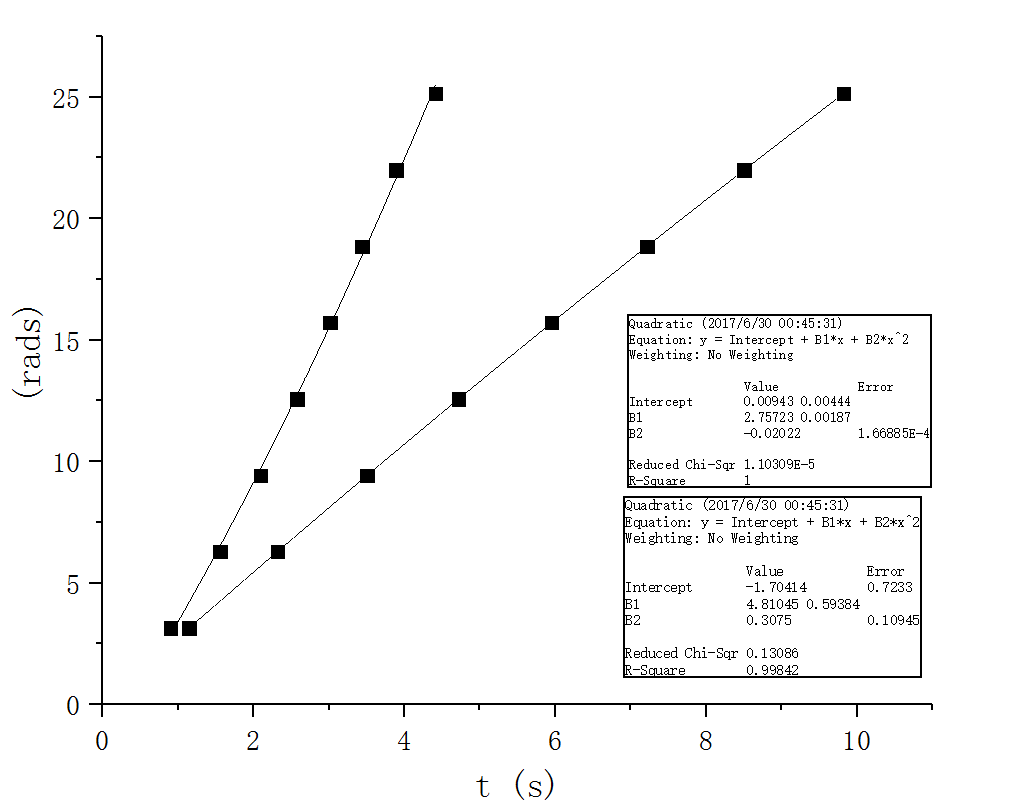
\includegraphics[width=1\linewidth]{P1.jpg}
\caption{Measurement data with error bars and a parabola fit for the relation between angle of rotation and time. The value for the obtained fit is two values of B2 in the tables.}
\end{figure}
From the fitting:
$$\beta_1=2\times{B2}=-0.0403\pm5.3684\times10^{-4}[rad/s^2]$$
$$\beta_2=2\times{B2}=0.0615\pm0.10945[rad/s^2]$$
$$I_1=\frac{mR(g-R\beta_2)}{\beta_2-\beta_1}=0.0203\pm3.4\times10^{-4}[kg\cdot{m^2}]$$

\subsubsection{Moment of Inertia of the Disk}
\begin{figure}[H]
\centering
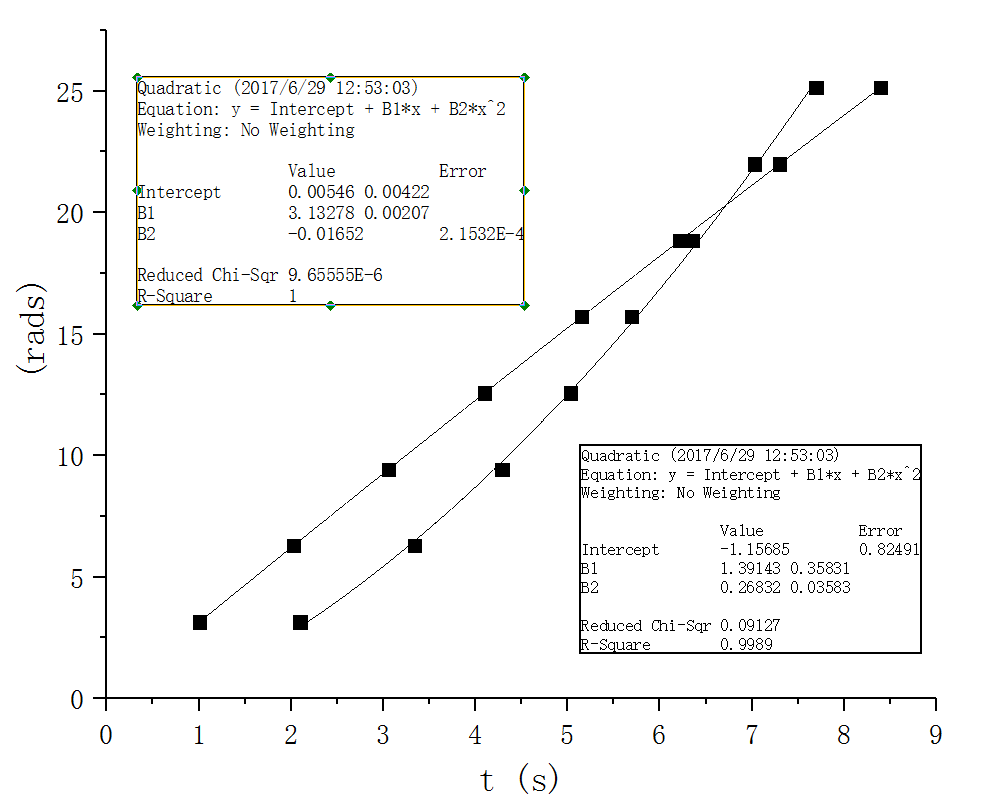
\includegraphics[width=1\linewidth]{P2.jpg}
\caption{Measurement data with error bars and a parabola fit for the relation between angle of rotation and time. The value for the obtained fit is two values of B2 in the tables.}
\end{figure}
From the fitting:
$$\beta_3=2\times{B2}=-0.0330\pm4.3064	\times10^{-4}[rad/s^2]$$
$$\beta_4=2\times{B2}=0.5366\pm0.0717[rad/s^2]$$
$$I_2=\frac{mR(g-R\beta_4)}{\beta_4-\beta_3}=0.0234\pm3\times10^{-4}[kg\cdot{m^2}]$$
$$I_{disk}=I_2-I_1=3.1\times10^{-3}\pm4.534\times10^{-4}[kg\cdot{m^2}]$$

\subsubsection{Moment of Inertia of the Hoop}
\begin{figure}[H]
\centering
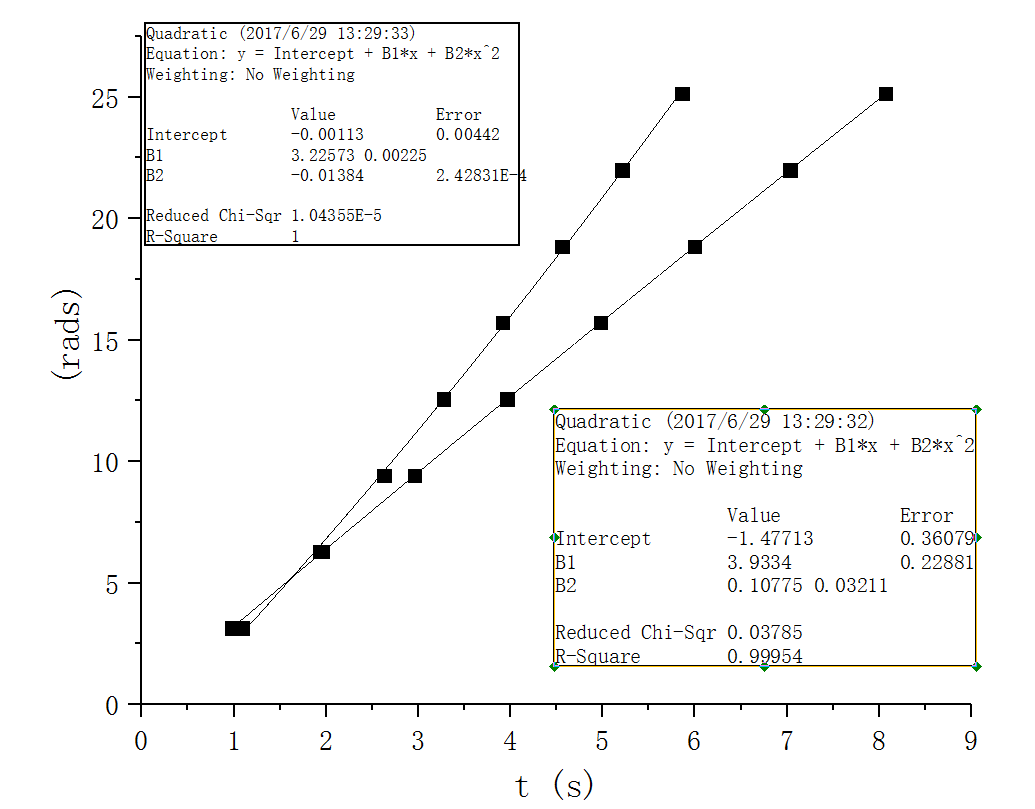
\includegraphics[width=1\linewidth]{P3.jpg}
\caption{Measurement data with error bars and a parabola fit for the relation between angle of rotation and time. The value for the obtained fit is two values of B2 in the tables.}
\end{figure}
From the fitting:
$$\beta_3=2\times{B2}=-0.0277\pm4.8566\times10^{-4}[rad/s^2]$$
$$\beta_4=2\times{B2}=0.2155\pm0.0642[rad/s^2]$$
$$I_2=\frac{mR(g-R\beta_4)}{\beta_4-\beta_3}=2.38\times10^{-2}\pm1.45\times10^{-2}[kg\cdot{m^2}]$$
$$I_{hoop}=I_2-I_1=3.45\times10^{-3}\pm1.25\times10^{-3}[kg\cdot{m^2}]$$

\subsubsection{Moment of Inertia of with Cylinder A in Hole\textcircled{1} and Cylinder B in Hole\textcircled{2}}
\begin{figure}[H]
\centering
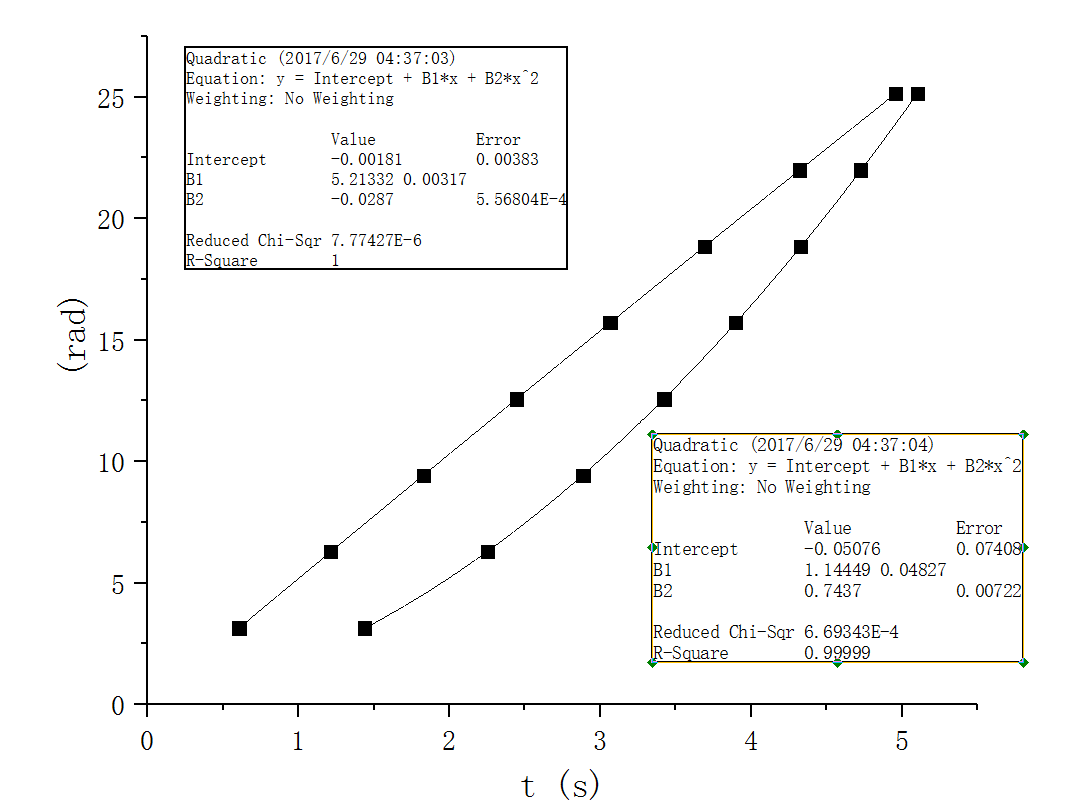
\includegraphics[width=1\linewidth]{P4.jpg}
\caption{Measurement data with error bars and a parabola fit for the relation between angle of rotation and time. The value for the obtained fit is two values of B2 in the tables.}
\end{figure}
From the fitting:
$$\beta_3=2\times{B2}=-0.0574\pm1.1136\times10^{-3}[rad/s^2]$$
$$\beta_4=2\times{B2}=1.4874\pm0.0144[rad/s^2]$$
$$I_2=\frac{mR(g-R\beta_4)}{\beta_4-\beta_3}=1.913\times10^{-2}\pm1.15\times10^{-4}[kg\cdot{m^2}]$$
$$I_{A1B2}=I_2-I_1=-1.17\times10^{-3}\pm3.589\times10^{-4}[kg\cdot{m^2}]$$

\subsubsection{Moment of Inertia of with Cylinder A in Hole\textcircled{3} and Cylinder B in Hole\textcircled{4}}
\begin{figure}[H]
\centering
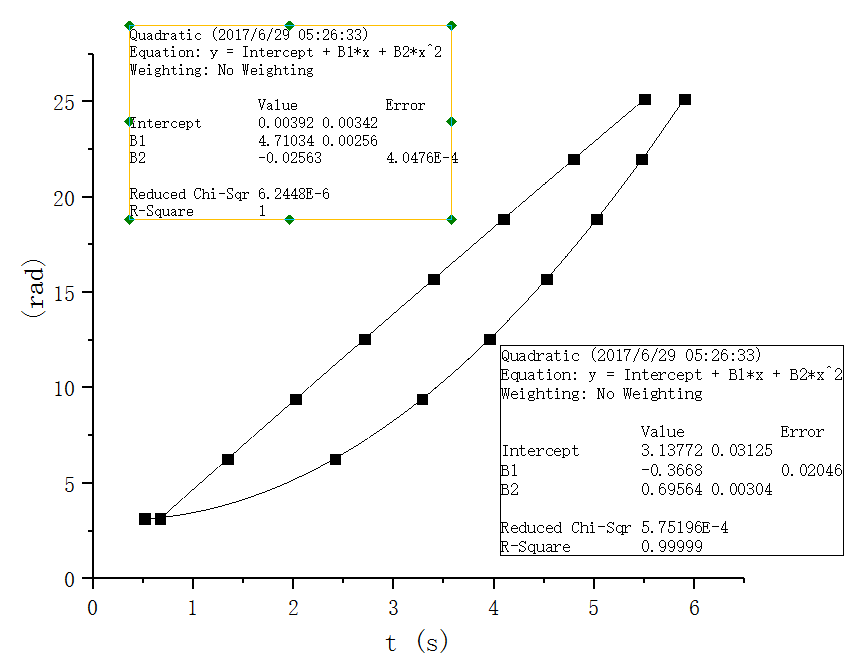
\includegraphics[width=1\linewidth]{P5.jpg}
\caption{Measurement data with error bars and a parabola fit for the relation between angle of rotation and time. The value for the obtained fit is two values of B2 in the tables.}
\end{figure}
From the fitting:
$$\beta_3=2\times{B2}=-0.0513\pm8.0952\times10^{-4}[rad/s^2]$$
$$\beta_4=2\times{B2}=1.3913\pm0.0061[rad/s^2]$$
$$I_2=\frac{mR(g-R\beta_4)}{\beta_4-\beta_3}=1.919\times10^{-2}\pm1.05\times10^{-4}[kg\cdot{m^2}]$$
$$I_{A3B4}=I_2-I_1=-1.11\times10^{-3}\pm3.558\times10^{-4}[kg\cdot{m^2}]$$

\section{Measurement Uncertainty Analysis}
\subsection{Range Measurement Uncertainty}
\subsubsection{Multiple measurements yield to type A uncertainty}
For multiple measurements' uncertainty:
$$\bar{X}=\frac{1}{n}\sum_{i=1}^nx_i$$
$$S_X=\sqrt{\frac{1}{n-1}\sum_{i=1}^n(x_i-\bar{X})^2}$$  
$$\bigtriangleup_A=\frac{S_Xt_{0.95}}{\sqrt{n}}$$
The value of $t_0.95$ and $\frac{t_{0.95}}{\sqrt{n}}$ are giving in Table 4 

\begin{table}[H]
\centering
\begin{tabular}{|l|l|l|l|l|l|l|l|l|l|l|l|}
\hline
n                         & 3    & 4    & 5     & 6    & 7     & 8     & 9     & 10    & 15    & 20    & $\ge100$   \\ \hline
$t_0.95$                  & 4.30 & 3.18 & 2.78  & 2.57 & 2.45  & 2.36  & 2.31  & 2.26  & 2.14  & 2.09  & $\le1.97$  \\ \hline
$\frac{t_0.95}{\sqrt{n}}$ & 2.48 & 1.59 & 1.204 & 1.05 & 0.926 & 0.834 & 0.770 & 0.715 & 0.553 & 0.467 & $\le0.139$ \\ \hline
\end{tabular}
\caption{The values of $t_{0.95}$ and $\frac{t_{0.95}}{\sqrt{n}}$}
\end{table}


\par The total uncertainty $u=\sqrt{(\bigtriangleup_A)^2+(\bigtriangleup_B)^2}$ and relative uncertainty $u_r=\frac{u}{\bar{X}}\times100\%$. For example, we can calculate the uncertainty of disk's diameter as the following process:
$$\bar{X}=\frac{1}{4}\sum_{i=1}^4x_i=24.000[cm]$$
$$S_X=\sqrt{\frac{1}{3}\sum_{i=1}^4(x_i-24.000)^2}=0.009$$   
$$\bigtriangleup_A=1.59{S_X}=0.014$$
$$\bigtriangleup_B=0.002[cm]$$
$$u=\sqrt{{0.014}^2+{0.002}^2}=0.015[cm]$$
$$u_r=\frac{0.015}{24.000}\times100\%=0.06\%$$
\subsubsection{Single measurement yields to type B uncertainty}
Since the calliper's resolution is 0.002[cm], $\bigtriangleup_B=\bigtriangleup_\varnothing=0.002[cm]$
When I measured the distance from holes to the center of the disk, I use the average value of the inner distance and external distance.
\begin{equation}
d=\frac{d_1+d_2}{2}
\end{equation} 
Since it's indirect measurement,its uncertainty is estimated:
$$u_d=\sqrt{(\frac{\partial{d}}{\partial{d_1}})^2{u_1}^2+(\frac{\partial{d}}{\partial{d_2}})^2{u_2}^2}=\sqrt{(\frac{1}{2})^2{(0.002[cm])}^2+(\frac{1}{2})^2{(0.002[cm])}^2}=0.0014[cm]$$
\subsubsection{The Final Uncertainty of Calliper Measurement}
\begin{table}[H]
\centering
\begin{tabular}{|r|c|c|c|}
\hline
\multicolumn{1}{|c|}{Object}                           & Average & $\pm$Uncertainty {[}cm{]} & Relative uncertainty \\ \hline
Disk $\varnothing$ {[}cm{]}        & 24.000  & 0.015                     & 0.06\%               \\ \hline
Hoop $\varnothing_1$ {[}cm{]}      & 21.349  & 0.133                     & 0.63\%               \\ \hline
Hoop $\varnothing_2$ {[}cm{]}      & 23.600  & 0.067                     & 0.29\%               \\ \hline
Cylinder A $\varnothing$ {[}cm{]}  & 2.993   & 0.011                     & 0.37\%               \\ \hline
Cylinder B $\varnothing$ {[}cm{]}  & 2.989   & 0.008                     & 0.26\%               \\ \hline
Cone pulley $\varnothing$ {[}cm{]} & 5.015   & 0.007                     & 0.14\%               \\ \hline
Hole \textcircled{1} d {[}cm{]}  & 4.508   & 0.0014                    & 0.03\%               \\ \hline
Hole \textcircled{2} d {[}cm{]}  & 4.508   & 0.0014                    & 0.03\%               \\ \hline
Hole \textcircled{3} d {[}cm{]}  & 5.993   & 0.0014                    & 0.02\%               \\ \hline
Hole \textcircled{4} d {[}cm{]}  & 5.985   & 0.0014                    & 0.02\%               \\ \hline
\end{tabular}
\caption{Uncertainty of calliper measurements}
\end{table}	

\subsection{Mass Measurements Uncertainty}
A single measurement for mass yields only type B uncertainty $\bigtriangleup_B=\bigtriangleup_\varnothing=0.1[g]. \\u=\bigtriangleup_B=0.1[g].$
\begin{table}[H]
\centering

\begin{tabular}{|r|c|c|c|}
\hline
\multicolumn{1}{|c|}{Object} & Mass  & $\pm$Uncertainty {[}g{]} & Relative uncertainty \\ \hline
Disk {[}g{]}                 & 490.2 & 0.1                      & 0.02\%               \\ \hline
Hoop {[}g{]}                 & 429.4 & 0.1                      & 0.02\%               \\ \hline
Cylinder A {[}g{]}           & 166.0 & 0.1                      & 0.06\%               \\ \hline
Cylinder B {[}g{]}           & 165.9 & 0.1                      & 0.06\%               \\ \hline
Weight {[}g{]}               & 54.5  & 0.1                      & 0.18\%               \\ \hline
\end{tabular}
\caption{Uncertainty of electronic balance measurements}
\end{table}

\subsection{Time Measurements Uncertainty}
A single measurement for time yields only type B uncertainty $\bigtriangleup_B=\bigtriangleup_\varnothing=0.0001[s]. \\u=\bigtriangleup_B=0.0001[s]$ and $u_r=0.004\%$
\subsection{Uncertainty of Theoretical Moment of Inertia}
The theoretical moment of inertia is calculated through other parameters measured so I should use the formula for combined uncertainty to estimate it. First, we should know its resolution and relative uncertainty.

\begin{table}[H]
\centering
\begin{tabular}{|c|c|c|}
\hline
Object                                                                                      & $u[kg\cdot{m^2}]$ & $u_r[\%]$ \\ \hline
With disk                                                                                   & $4.47\times10^{-6}$             & 0.13      \\ \hline
With Hoop                                                                                   & $3.66\times10^{-5}$              & 0.67      \\ \hline
\begin{tabular}[c]{@{}c@{}}Cylinder A in hole \\ \textcircled{1} and Cylinder \\ B in hole \textcircled{2}\end{tabular} & $1.6\times10^{-5}$              & 2.2     \\ \hline
\begin{tabular}[c]{@{}c@{}}Cylinder A in hole \\ \textcircled{3} and Cylinder \\ B in hole \textcircled{4}\end{tabular} & $5.06\times10^{-7}$ \          & 0.04      \\ \hline
\end{tabular}
\caption{Uncertainty of theoretical moment of inertia}
\end{table}
\subsubsection{Calculation of uncertainty of theoretical $I_{disk}$}
$$u=\sqrt{(\frac{\partial{I}}{\partial{m}}\cdot{u_m})^2+(\frac{\partial{I}}{\partial{R}}\cdot{u_R})^2}=\sqrt{(\frac{R^2}{2}\cdot{u_m})^2+(MR\cdot{u_R})^2}=4.47\times10^{-6}[kg\cdot{m^2}]$$
$$u_r=\frac{u}{I_{disk}}\times100\%=0.13\%$$
\subsubsection{Calculation of uncertainty of theoretical $I_{hoop}$}
$$u=\sqrt{(\frac{\partial{I}}{\partial{m}}\cdot{u_m})^2+(\frac{\partial{I}}{\partial{R_1}}\cdot{u_{R_1}})^2+(\frac{\partial{I}}{\partial{R_2}}\cdot{u_{R_2}})^2}$$
$$=\sqrt{(\frac{(R_1+R_2)^2}{2}\cdot{u_m})^2+(MR_1\cdot{u_{R_1}})^2+(MR_2\cdot{u_{R_2}})^2}=3.66\times10^{-5}[kg\cdot{m^2}]$$
$$u_r=\frac{u}{I_{hoop}}\times100\%=0.67\%$$
\subsubsection{Calculation of uncertainty of theoretical $I_{A1B2}$ and $I_{A3B4}$}
When Cylinder A is placed at \textcircled{1} and Cylinder B is placed at \textcircled{2} Then $$u_{A1B2}=\sqrt{(\frac{\partial{I_{A1B2}}}{\partial{m_A}}\cdot{u_{m_A}})^2+(\frac{\partial{I_{A1B2}}}{\partial{m_B}}\cdot{u_{m_B}})^2+\frac{\partial{I_{A1B2}}}{\partial{d_1}}\cdot{u_{d_1}})^2+\frac{\partial{I_{A1B2}}}{\partial{d_2}}\cdot{u_{d_2}})^2+\frac{\partial{I_{A1B2}}}{\partial{u_A}}\cdot{u_A})^2+(\frac{\partial{I_{A1B2}}}{\partial{u_B}}\cdot{u_B})^2}$$
$$=1.6\times10^{-5}[kg\cdot{m^2}]$$

When Cylinder A is placed at \textcircled{3} and Cylinder B is placed at \textcircled{4} Then $$u_{A1B2}=\sqrt{(\frac{\partial{I_{A1B2}}}{\partial{m_A}}\cdot{u_{m_A}})^2+(\frac{\partial{I_{A1B2}}}{\partial{m_B}}\cdot{u_{m_B}})^2+\frac{\partial{I_{A3B4}}}{\partial{d_3}}\cdot{u_{d_3}})^2+\frac{\partial{I_{A3B4}}}{\partial{d_4}}\cdot{u_{d_4}})^2+\frac{\partial{I_{A3B4}}}{\partial{u_A}}\cdot{u_A})^2+(\frac{\partial{I_{A3B4}}}{\partial{u_B}}\cdot{u_B})^2}$$
$$=5.06\times10^{-7}[kg\cdot{m^2}]$$
\subsection{Uncertainty of Angular Acceleration and Deceleration}
Since we can get the angular acceleration and deceleration through image fitting, the software "origin" can also give us their uncertainty.

\begin{table}[H]
\centering
\begin{tabular}{|c|c|c|}
\hline
\multicolumn{3}{|c|}{Uncertainty of $\beta$ $[rad/s^2]$} \\ \hline
                & Deceleration    & Acceleration    \\ \hline
Empty table     & $1.6689\times10^{-4}$          & 0.1095          \\ \hline
With disk       & $2.1532\times10^{-4}$          & 0.0358          \\ \hline
With hoop       & $2.4283\times10^{-4}$         & 0.0321          \\ \hline
\begin{tabular}[c]{@{}c@{}}Cylinder A in hole \\ \textcircled{1} and Cylinder \\ B in hole \textcircled{2}\end{tabular}      & $5.568\times10^{-4}$          & 0.0072          \\ \hline
\begin{tabular}[c]{@{}c@{}}Cylinder A in hole \\ \textcircled{3} and Cylinder \\ B in hole \textcircled{4}\end{tabular}     & $4.0476\times10^{-4}$          & 0.003 \\ \hline
\end{tabular}
\caption{Uncertainty of $\beta$}
\end{table}

\subsection{Uncertainty of Measured Moment of Inertia}

\begin{table}[H]
\centering
\begin{tabular}{|c|c|c|}
\hline
\multicolumn{3}{|c|}{Uncertainty of $I$} \\ \hline
                & $u [kg\cdot{m^2}]$    & $u_r[\%]$   \\ \hline
Empty table     & $3.4\times10^{-4}$          & 1.67          \\ \hline
With disk       & $4.534\times10^{-4}$          & 14.6        \\ \hline
With hoop       & $1.25\times10^{-2}$         & 36.23          \\ \hline
\begin{tabular}[c]{@{}c@{}}Cylinder A in hole \\ \textcircled{1} and Cylinder \\ B in hole \textcircled{2}\end{tabular}      & $3.589\times10^{-4}$          & 30.67 \\ \hline
\begin{tabular}[c]{@{}c@{}}Cylinder A in hole \\ \textcircled{3} and Cylinder \\ B in hole \textcircled{4}\end{tabular}     & $3.558\times10^{-4}$          & 32.05 \\ \hline
\end{tabular}
\caption{Uncertainty of measured moment of inertia}
\end{table}
To calculate the uncertainty of $I_0$
$$u_{I_0}=\sqrt{(\frac{\partial{I_0}}{\partial{m}}u_m)^2+(\frac{\partial{I_0}}{\partial{R}}u_R)^2+(\frac{\partial{I_0}}{\partial{\beta_1}}u_{\beta_1})^2+(\frac{\partial{I_0}}{\partial{\beta_2}}u_{\beta_2})^2+(\frac{\partial{I_0}}{\partial{g}}u_g)^2}$$
$$=\sqrt{(\frac{(g-R\beta_2)R}{\beta_2-\beta_1}u_m)^2+(\frac{(g-2R\beta_2)m}{\beta_2-\beta_1}u_R)^2+(\frac{(g-R\beta_2)mR}{(\beta_2-\beta_1)^2}u_{\beta_1})^2+(\frac{(g-R\beta_1)mR}{(\beta_2-\beta_1)^2}u_{\beta_2})^2+(\frac{-mR}{\beta_2-\beta_1}u_g)^2}$$
$$=3.4\times10^{-4}$$
$$u_{r {I_0}}=\frac{u_{I_0}}{I_0}\times100\%1.67\%$$
Similarly, the resolution and relative uncertainty of $I_{disk}$, $I_{hoop}$, $I_{A1B2}$, and $I_{A3B4}$ can be calculated as $u_{I_0}$ and $u_{r {I_0}}$
$$u_{Idisk}=4.534\times10^{-4}[kg\cdot{m^2}]$$
$$u_{r_{disk}}=14.6\%$$
$$u_{Ihoop}=1.25\times10^{-2}[kg\cdot{m^2}]$$
$$u_{r_{hoop}}=36.23\%$$
$$u_{IA1B2}=3.589\times10^{-4}[kg\cdot{m^2}]$$
$$u_{r_{A1B2}}=30.67\%$$
$$u_{IA3B4}=3.558\times10^{-4}[kg\cdot{m^2}]$$
$$u_{r_{A3B4}}=32.05\%$$
\section{Conclusion and Discussion}
\subsection{Conclusion}
In this experiment, I use constant-torque method to measure the moment of inertia of a rigid body. Parallel axis theorem can also be verified by comparing my measured moment of inertia to my theoretically calculated data.
\par Through this exercise, I have a rough idea about the concept of rigid body, its moment of inertia, rotational motion, and parallel axis theorem. In addition, I learn how to use the calliper, electronic balance, and timer to measure relative physics quantity with high accuracy after this experiment.  
\par Moreover, uncertainty analysis is very important in the exercise. It's the first time I analyse the uncertainty of physical quantities. In the exercise, lots of data are recorded, which leads to many calculation of uncertainty. When I use the data measured, I must first calculate the random errors and systematic errors then I can get the total measurement uncertainty.
\subsection{Discussion}
\subsubsection{Error Analysis}
\begin{table}[H]
\centering

\begin{tabular}{|c|c|c|c|}
\hline
\multicolumn{1}{|c|}{Object} & Measured I $kg\cdot{m^2}$  & Theoretical I ${kg\cdot{m^2}}$ & Relative error \\ \hline
With disk                 & $3.1\times10^{-3}\pm4.534\times10^{-4}$                      & $3.529\times10^{-3}\pm4.47\times10^{-6}$&12\%               \\ \hline
With hoop         & $3.45\times10^{-3}\pm1.25\times10^{-2}$ & $5.435\times10^{-3}\pm3.66\times10^{-5}$ & 36\%               \\ \hline
\begin{tabular}[c]{@{}c@{}}Cylinder A in hole \\ \textcircled{1} and Cylinder \\ B in hole \textcircled{2}\end{tabular}          & $-1.17\times10^{-3}\pm3.589\times10^{-4}$ & $7.116\times10^{-4}\pm1.6\times10^{-5}$                      & 160.8\%               \\ \hline
\begin{tabular}[c]{@{}c@{}}Cylinder A in hole \\ \textcircled{3} and Cylinder \\ B in hole \textcircled{4}\end{tabular}                & $-1.11\times10^{-3}\pm3.558\times10^{-4}$  & $1.228\times10^{-3}\pm5.06\times10^{-7}$                      & 190\%               \\ \hline
\end{tabular}
\caption{Relative error of moment of inertia}
\end{table}

From the table of moment of inertia, I can observe the relative error is quite bigger than excepted, especially when I put the cylinders on the holes. As a result, the error analysis is extremely important.
\par Since the errors of disk and hoop's moment of inertia are not so big, I guess my calculation of $I_0$ is not. The main problem lies in the calculation of $I_A1B2$ and $I_A3B4$, because it should never be negative value. I think external force might be exerted on equipments during my measurement and cause the errors. 
\par What's more, I found my timer is very unstable in my experiment because sometimes it'll miss the data or record the time twice. It caused me a lot of trouble. For sake of stability, I did the first three measurement again but I can't repeat the last two due to the limited time, so it may lead big errors in my data.

\subsection{Suggestions and Improvement}
\begin{enumerate}
\item Give the table an appropriate initial angular velocity. If it's too fast or too slow, it will lead to huge uncertainty and lack accuracy.
\item Never exert an external force on the materials because it will change the angular acceleration or deceleration measured. 
\item Better timer is preferred.
\item I should improve my efficiency and save time in my experiment.
\end{enumerate}
\section{Data Sheet}
Data sheet is attach to the report
\section{Reference}
\par Young, H.D., Freedman R.A. University Physics. Chapter 9,10.
\par Qin Tian, Zeng Ming, Zhao Xijian, Krzyzosiak,M. Lab Manual of Exercise 1.
\par Qin Tian, Zeng Ming, Zhao Xijian, Krzyzosiak,M. Handbook-Uncertainty Analysis.
\end{document}